\chapter{Desenho do Processo Macro} \label{cha:desenhomacro}
Neste capítulo são apresentados os diagramas de atividades das principais funcionalidades que serão implementados no aplicativo.

%DUVIDA: MTO PEQUENO SÓ ATIVIDADES?

A atividade "Buscar Produto", diagramada na figura \autoref{fig:atividade_comparar}, na qual o usuário insere um termo de pesquisa para encontrar produtos de interesse. Em seguida, o sistema executa a ação de "Pesquisar Produto", onde são consultadas as lojas cadastradas para encontrar produtos que correspondam ao termo de pesquisa. Após a pesquisa, o sistema verifica se foram encontrados produtos. Se sim, o fluxo segue para a atividade "Comparar Preços", na qual os preços dos produtos encontrados são coletados e comparados entre as diferentes lojas ou fontes disponíveis. Durante essa comparação, o sistema identifica o melhor preço para cada produto.

Ao final da atividade de comparar preços, o sistema pode exibir os resultados da comparação ao usuário, mostrando os produtos encontrados, seus preços em diferentes lojas e destacando o melhor preço disponível. Isso ajuda o usuário a tomar uma decisão informada sobre qual produto comprar com base no preço mais atrativo.

A atividade de visualizar ou alterar sugestões de preços, diagramada na figura \autoref{fig:atividade_sugestoes}, tem início na etapa de visualização de detalhes do produto. Caso o produto já tenha um preço cadastrado o usuário pode avaliar a sugestão ou inserir outra. Essa atualização é fundamental para garantir que os usuários recebam informações precisas e atualizadas sobre os preços dos produtos que estão monitorando ou pesquisando.

\imagem{DIAGRAMA DE ATIVIDADES COMPARAR PREÇOS}{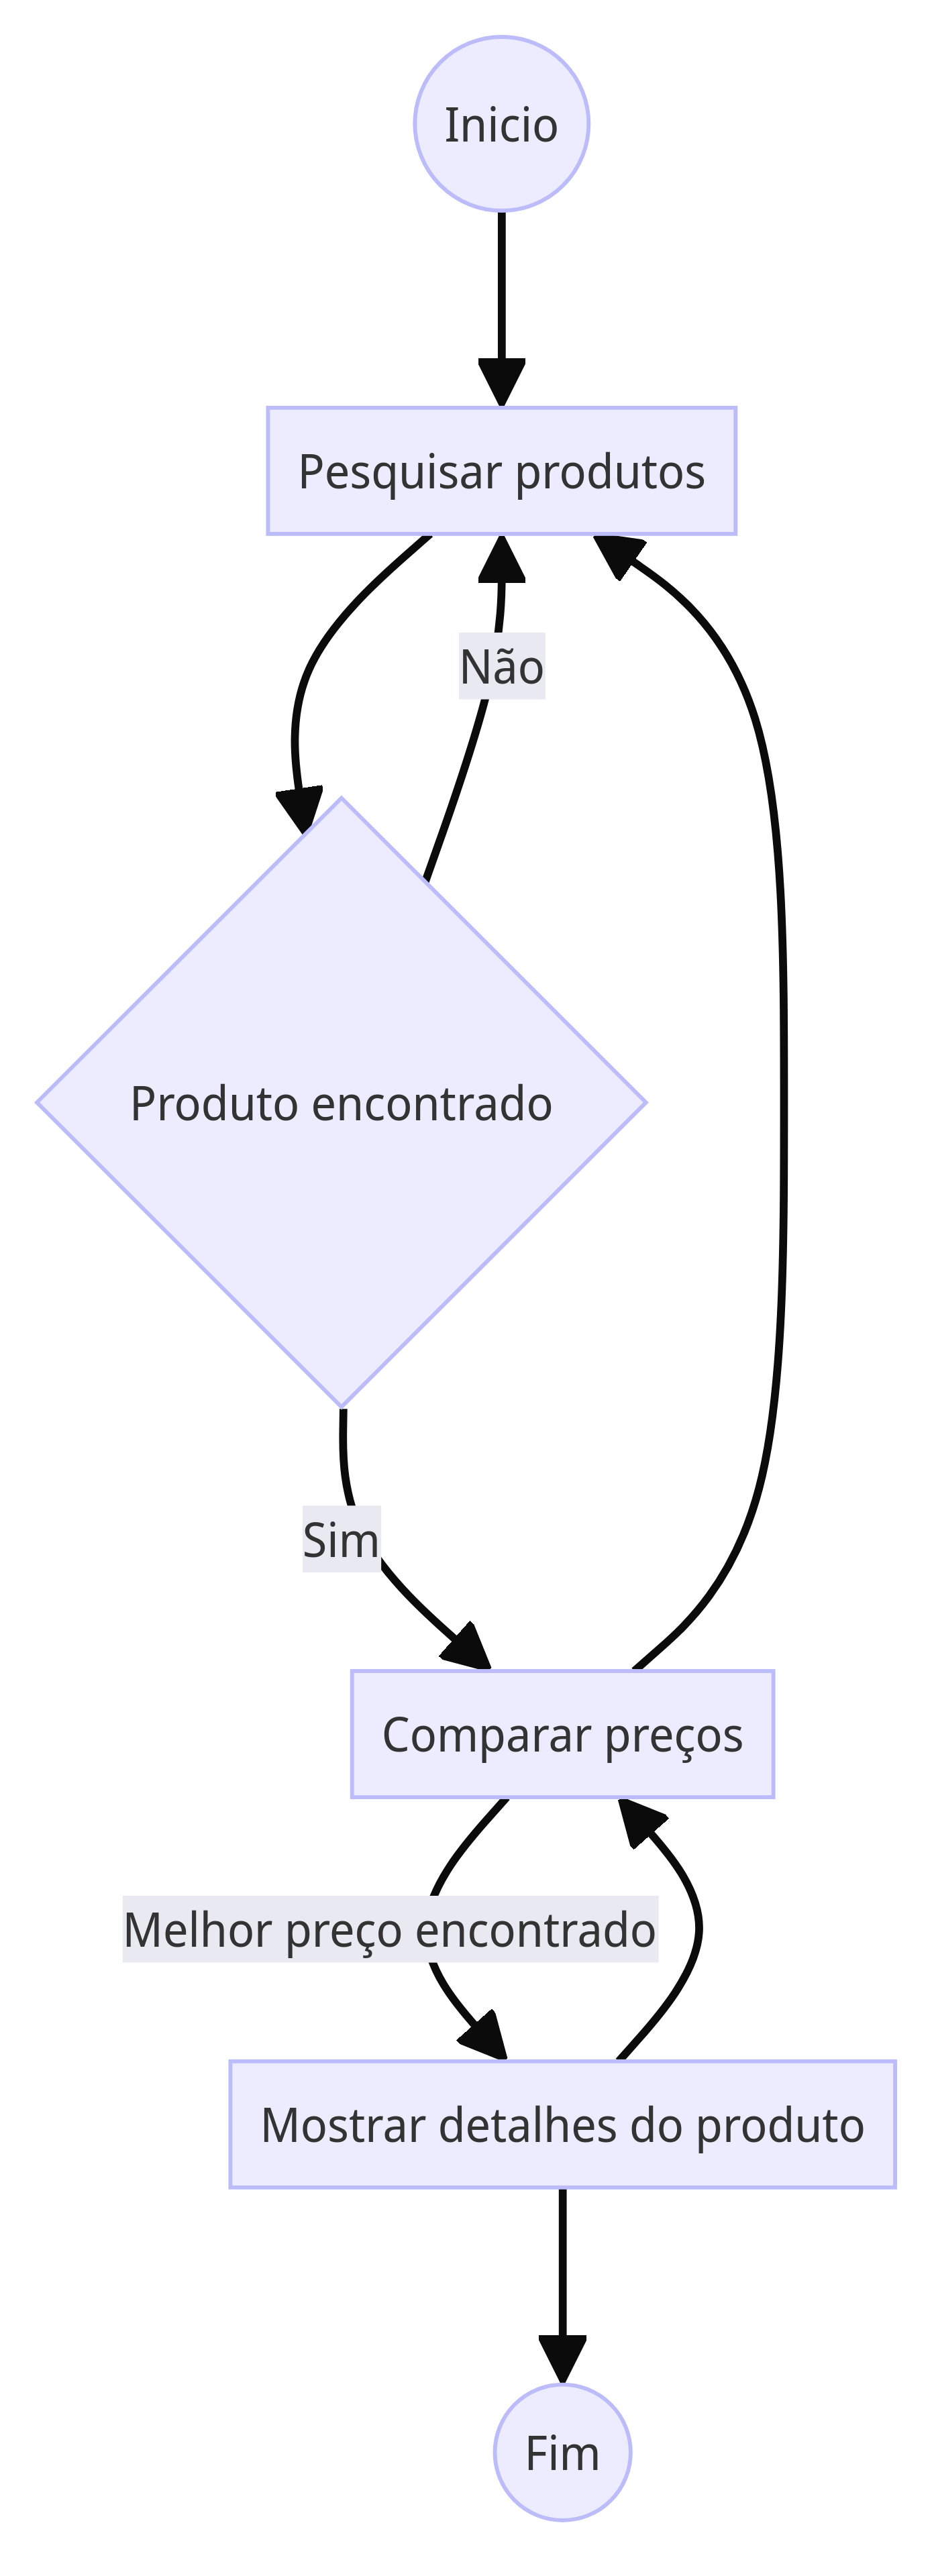
\includegraphics[width = 60mm]{fig/atividade/atividade1.png}}{O Autor (2024)}{fig:atividade_comparar}{nota(s)}{legenda(s)}

\imagem{DIAGRAMA DE ATIVIDADES SUGESTÕES PREÇO}{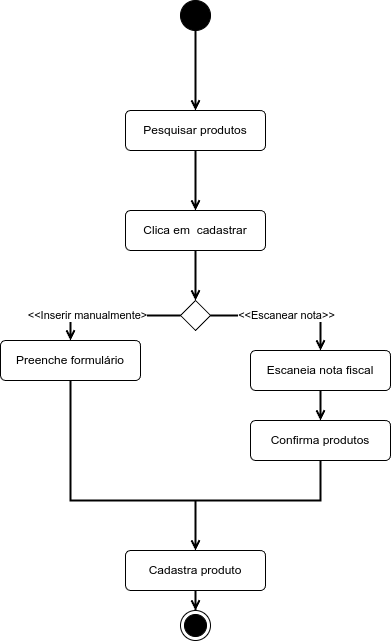
\includegraphics[width = 120mm]{fig/atividade/atividade2.png}}{O Autor (2024)}{fig:atividade_sugestoes}{nota(s)}{legenda(s)}